% \pagebreak[4]
% \hspace*{1cm}
% \pagebreak[4]
% \hspace*{1cm}
% \pagebreak[4]

\chapter{Cost Effective Study Design in an African Population}
\ifpdf
    \graphicspath{{Chapter1/Chapter1Figs/PNG/}{Chapter1/Chapter1Figs/PDF/}{Chapter1/Chapter1Figs/}}
\else
    \graphicspath{{Chapter1/Chapter1Figs/EPS/}{Chapter1/Chapter1Figs/}}
\fi

%A \acrlong{SNP} is abbreviated abbreviated \acrshort{SNP}.
A \gls{SNP} is a \Gls{SNP} is a \GLS{SNP}. Testing glossary.

\section{Introduction}
\section{Data Description}
Omni/HiSeq Sample count table. Omni/HiSeq SNP count table. Sample coverage table.
\section{Methods}
\subsection{SNP Chip Array QC}
\subsection{Sequencing}
The ability to sequence depends on the sequence content and the ability to map depends on the uniqueness of the sequence and the presence and length of indels.
\subsection{Downsampling}
GATK PrintReads\cite{DePristo2011}
\subsection{BAM pre-processing}
We carry out base quality score recalibration. Base quality doesn't have any impact on indel realignment, so it wouldn't make a difference. But having reads realigned properly improves the base recalibration model because it reduces the number of artifactual SNPs.
We mark duplicates for exclusion with Picard, because sequencing errors are otherwise propagated in duplicates leading to false positive variant calls.
\subsubsection{Realignment around INDELs}
Improves accuracy of downstream processing steps. Avoid mappers mis-aligning with mismatches. Regions that need to be realigned are identified with GATK RealignerTargetCreater and the actual realignment is performed with GATK IndelRealigner.
%Ask Martin if he uses the -known flag, which is accurate for ~90-95% of indels. Check if info in BAM header.
%Recommendations here: https://www.broadinstitute.org/gatk/guide/article?id=1247
\subsection{Variant Calling}
Also include samtools, FreeBayes and Platypus.
Remember that HC does INDEL realignment on the fly...
Minimum read mapping quality required to consider a read for analysis with the HaplotypeCaller (HCMappingQualityFilter) (--min_mapping_quality_score 20)
HC DuplicateReadFilter
Target coverage threshold for downsampling to coverage HC --downsampling_type BY_SAMPLE --downsample_to_coverage 250
Minimum base quality required to consider a base for calling --min_base_quality_score 10 (UG17)
The minimum phred-scaled confidence threshold at which variants should be called --standard_min_confidence_threshold_for_calling
The minimum phred-scaled confidence threshold at which variants should be emitted (and filtered with LowQual if less than the calling threshold) --standard_min_confidence_threshold_for_emitting
HC only maxNumHaplotypesInPopulation 128
max_alternate_alleles 6
%INDELs, especially those disrupting protein-coding regions of the genome, have been strongly associated with human diseases.
%http://www.ncbi.nlm.nih.gov/clinvar?term=human%5Borgn%5D
\subsection{Variant Filtering}
VQSLOD is the log odds ratio of being a true variant versus being false.
\subsection{Genotype refinement}
1000G because small sample size!
\subsection{WGS QC}
\section{Results}
\subsection{Comparison of variant calling and refinement methods}
\subsection{Comparison of variant calling software}
\subsection{Comparison of refinement software and reference panels}
\subsection{Statistics after downsampling}
Lots of table and figures. Copy/Paste from Word.
\subsection{Apparent sample size}
\section{Discussion}
\section{Conclusions}

%\section{First Paragraph}
And now I begin my first chapter here ...

Here is an equation\footnote{the notation is explained in the nomenclature section :-)}:
\begin{eqnarray}
CIF: \hspace*{5mm}F_0^j(a) &=& \frac{1}{2\pi \iota} \oint_{\gamma} \frac{F_0^j(z)}{z - a} dz
\end{eqnarray}
\nomenclature[zcif]{$CIF$}{Cauchy's Integral Formula}                                % first letter Z is for Acronyms 
\nomenclature[aF]{$F$}{complex function}                                                   % first letter A is for Roman symbols
\nomenclature[gp]{$\pi$}{ $\simeq 3.14\ldots$}                                             % first letter G is for Greek Symbols
\nomenclature[gi]{$\iota$}{unit imaginary number $\sqrt{-1}$}                      % first letter G is for Greek Symbols
\nomenclature[gg]{$\gamma$}{a simply closed curve on a complex plane}  % first letter G is for Greek Symbols
\nomenclature[xi]{$\oint_\gamma$}{integration around a curve $\gamma$} % first letter X is for Other Symbols
\nomenclature[rj]{$j$}{superscript index}                                                       % first letter R is for superscripts
\nomenclature[s0]{$0$}{subscript index}                                                        % first letter S is for subscripts

%\section{Second Paragraph}
and here I write more ...\cite{texbook}

%\subsection{sub first paragraph}
... and some more ...

Now I would like to cite the following: \cite{latex} and \cite{texbook}
and \cite{Rud73}.

I would also like to include a picture ...

\begin{figure}[!htbp]
  \begin{center}
    \leavevmode
    \ifpdf
      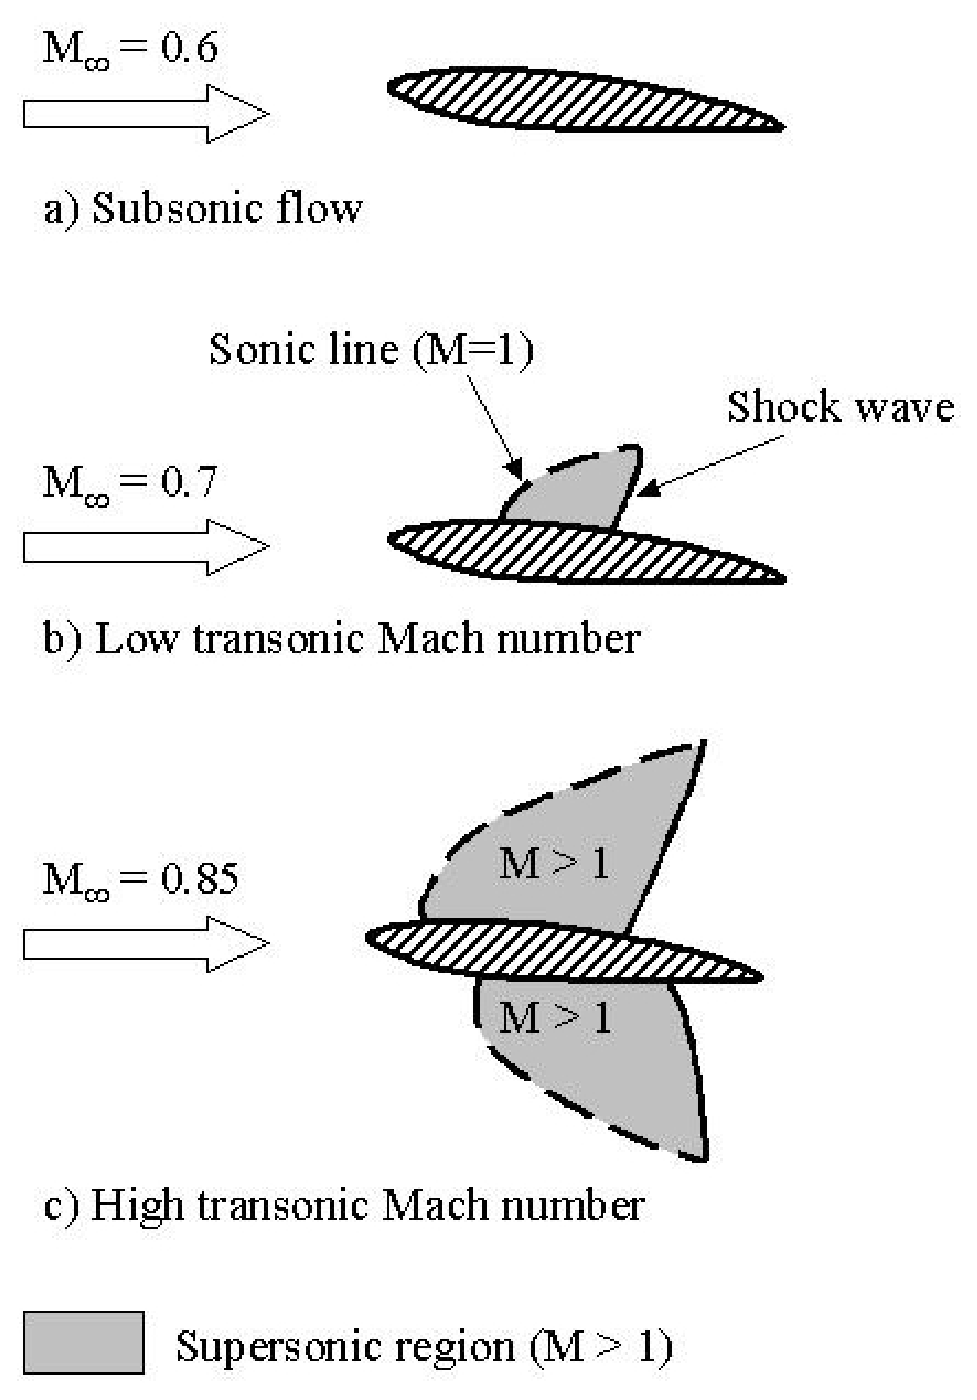
\includegraphics[height=6in]{aflow}
    \else
      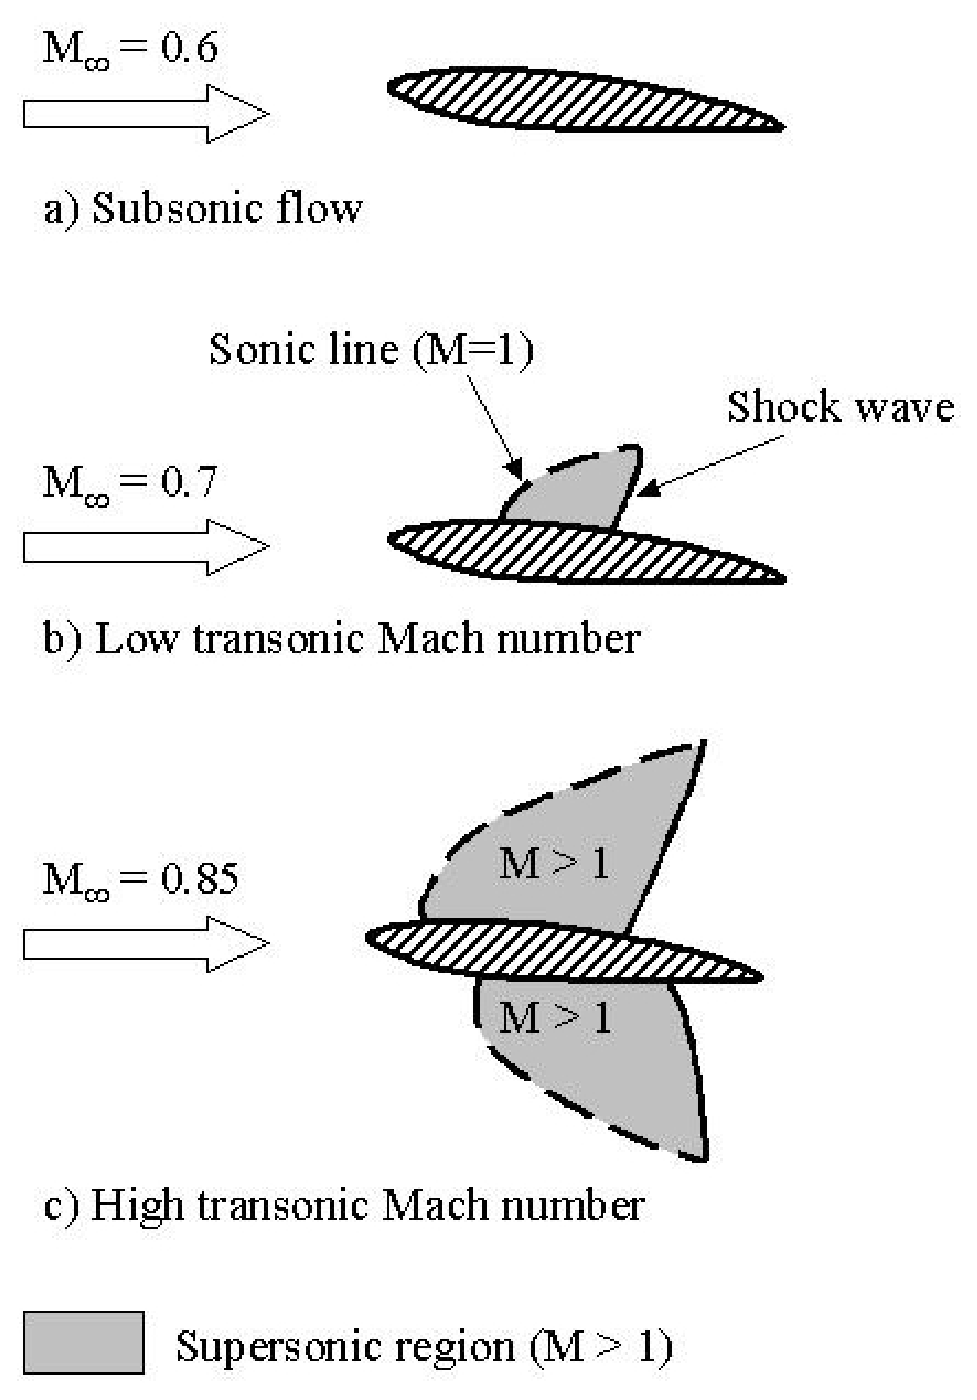
\includegraphics[bb = 92 86 545 742, height=6in]{aflow}
    \fi
    \caption{Airfoil Picture}
    \label{FigAir}
  \end{center}
\end{figure}

% above code has been macro-fied in Classes/MacroFile.tex file
%\InsertFig{\IncludeGraphicsH{aflow}{6in}{92 86 545 742}}{Airfoil Picture}{FigAir}

So as we have now labelled it we can reference it, like so (\ref{FigAir}) and it
is on Page \pageref{FigAir}. And as we can see, it is a very nice picture and we
can talk about it all we want and when we are tired we can move on to the next
chapter ...

I would also like to add an extra bookmark in acroread like so ...
\ifpdf
  \pdfbookmark[2]{bookmark text is here}{And this is what I want bookmarked}
\fi
% ------------------------------------------------------------------------


%%% Local Variables: 
%%% mode: latex
%%% TeX-master: "../thesis"
%%% End: 
